\documentclass[12pt, letterpaper]{article}
\usepackage[ngerman]{babel}
\usepackage{graphicx}
\usepackage{wrapfig}
\usepackage{titlesec}
\usepackage{geometry}
\usepackage[font=scriptsize]{caption}
\usepackage{blindtext}
\usepackage{hyperref}
\usepackage{tabularx}
\usepackage{subcaption}
\usepackage{verbatim}
\usepackage{fancyvrb}
\usepackage{listings}
\usepackage{xcolor}
\usepackage{multirow}
\usepackage{array} % Für die Spaltenbreitenanpassung
\usepackage{booktabs} % Für schönere Tabellen
\usepackage{geometry}
\usepackage{arydshln}
\usepackage{colortbl}
\usepackage{forest}
\usepackage{caption}
\usepackage{pifont}
\usepackage{amssymb}
\usepackage{enumitem}
\renewcommand{\lstlistlistingname}{Programmcode}

\geometry{a4paper, margin=2cm}
\hypersetup{
  colorlinks = true,
  linkcolor = black,
  urlcolor = blue,
}

% \captionsetup{justification=raggedright,singlelinecheck=false}
\geometry{
 a4paper,
 total={170mm,257mm},
 left=20mm,
 top=20mm,
 }
%  \titleformat{\section}[display]
%    {\normalfont\bfseries}{}{0pt}{\huge}

\lstdefinestyle{py}{
    language=Python,
    backgroundcolor=\color{white},
    keywordstyle=\color{blue}\bfseries,        % Default Python keywords
    commentstyle=\color{brown}\bfseries,         % Comments
    stringstyle=\color{brown},                 % Strings
    numberstyle=\tiny\color{gray},             % Line numbers
    basicstyle=\ttfamily\small,                % Base font
    identifierstyle=\color{black},             % Default for variable names
    keywordstyle=[2]\color{cyan},              % Functions
    keywordstyle=[3]\color{purple},            % Types
    breaklines=true,
    showstringspaces=false,
    tabsize=4,
    captionpos=b,
    %numbers=left,
    %numbersep=10pt,
    frame=single
}

% Define specific keywords
\lstset{
    morekeywords={import, from, def, return},  % Default Python keywords
    morekeywords=[2]{print, println, len, range, input}, % Functions
    morekeywords=[3]{int, float, str, list, dict, bool} % Types
}


\lstdefinestyle{cpp}{
    language=C,
    backgroundcolor=\color{white},
    keywordstyle=\color{blue}\bfseries,        % Standard Keywords
    commentstyle=\color{green}\itshape,        % Kommentare
    stringstyle=\color{orange},                % Strings
    numberstyle=\tiny\color{gray},             % Zeilennummern
    basicstyle=\ttfamily\small,                % Basis-Schriftart
    identifierstyle=\color{black},             % Standard für Variablennamen
    keywordstyle=[2]\color{cyan},              % Funktionen
    keywordstyle=[3]\color{purple},            % Typen
    breaklines=true,
    showstringspaces=false,
    tabsize=4,
    captionpos=b,
    %numbers=left,
    %numbersep=10pt,
    frame=single
}

% Spezifische Keywords definieren
\lstset{
    morekeywords={if, else, while, return},         % Standard C-Keywords
    morekeywords=[2]{printf, scanf, main, malloc},  % Funktionen (inkl. malloc)
    morekeywords=[3]{int, float, char, double}      % Typen
}

%\lstset{style=pycharm-light}

  
\usepackage{lipsum}  
\graphicspath{ {./Bilder/} }
\author{Oleksii Baida}
\date{Mai 2024}
\begin{document}
\begin{titlepage}
  
\includegraphics[width = 0.25\pdfpagewidth]{./Bilder/FHDO.jpg}
  \begin{center}
    
    \huge \textbf{\textsf{Bachelorarbeit}} \\
    \vspace{3cm}
    \large \textbf{Oleksii Baida}\\
    \textbf{Matrikelnummer 7210384}\\
    \vspace{3cm}
    \large \textbf{Sicherheits- \& Steuerungssytem für das Haus}\\
    \vspace{1cm}
    \large \textbf{Bericht}\\
    \vspace{1cm}
    \today
  \end{center}
\end{titlepage}

\tableofcontents
\pagebreak

\section{Einleitung}
\par In einer Welt, die zunehmend von vernetzten Geräten und dem Internet der Dinge geprägt ist, wird die Entwicklung effizienter und benutzerfreundlicher Systeme zur Steuerung und Überwachung von Gebäuden immer relevanter. Im Jahr 2024 wurde in Deutschland die Anzahl von über 19 Millionen Haushalten, die ein oder mehrere smarte Geräte besaßen, verzeichnet. Es wird prognostiziert, dass sich diese Zahl innerhalb der nächsten drei Jahre verdoppeln wird \cite{statita_smhomes}.
\par Moderne Steuerungs- und Sicherheitssysteme tragen zur Effizienzsteigerung und Ressourcenschonung bei. Laut Günther Ohland, Vorstandsmitglied des Branchenverbands "Smarthome Initiative Deutschland", ermöglichen diese Systeme eine Reduktion des Heizenergieverbrauchs um 20 bis 30 Prozent \cite{spiegel_heizung}. Die Kosten für die smarte Technik rechnen sich in der Regel nach zwei Jahren. Die Systeme übernehmen ein Teil der täglichen Aufgaben, wie das Ein- und Ausschalten des Lichts, die Reglung der Raumtemperatur oder das Aufräumen des Hauses etc. Der Aufgabenbereich der Systeme ist dabei nur nach den Bedürfnissen der Benutzerinnen und Benutzer abgegrenzt.
\par Im Rahmen meiner Bachelorarbeit wird ein System zur Steuerung und Überwachung des Hauses entwickelt. Das Ziel dieser Arbeit ist die Erstellung einer Schnittstelle, die die Interaktion des Benutzers mit den Geräten in seinem Haushalt ermöglicht und den Benutzer über gefährliche Vorgänge in seinem Haus informiert. 
\par Im Rahmen der Entwicklung dieses Systems wurden die aktuellen Technologien zur Erstellung eines Webinterfaces und zur Kommunikation zwischen den Geräten eingesetzt. \textbf{TODO Kurz erklären was in Kapitel 2,3,4,5 ... erklärt wird}

\newpage
\section{Grundlagen \& Theorie}
\par In diesem Abschnitt werden die technischen Spezifikationen der verwendeten Komponenten und Technologien detailliert beschrieben.
  \subsection{Hardware}
  \par Das Projekt umfasst verschiedene Hardware-Komponenten, darunter Mikrocontroller, Sensoren und einen Einplatinencomputer.
  \subsubsection{Arduino Uno}
    \par Der Arduino Uno ist ein Mikrocontroller-Board, das sich besonders für die Erfassung und Verarbeitung von Sensordaten eignet. Aufgrund seiner einfachen Programmierbarkeit und vielseitigen Schnittstellen wird es häufig in eingebetteten Systemen sowie in IoT-Anwendungen eingesetzt.
    \par Das Herz des Boards bildet der Mikrocontroller ATmega328P, der über Flash-Speicher und EEPROM{Electrically Erasable Programmable Read-Only Memory} verfügt. Das EEPROM ermöglicht die nichtflüchtige Speicherung von Daten, so dass diese auch nach dem Ausschalten des Gerätes erhalten bleiben.
    \par Die technischen Spezifikationen des Arduino Uno sind in Tabelle \ref{tab:arduinounotd} dargestellt.
    \begin{table}[h]
      \centering
      \begin{tabular}{|l|l|}
          \hline
          Modell                         & Arduino Uno                \\ \hline
          Mikrocontroller                & ATmega328P                      \\ \hline
          Taktfrequenz                   & 16 MHz                          \\ \hline
          Eingangsspannung               & 12 V                          \\ \hline
          Digital Pins                   & 14           \\ \hline
          Analoge Eingänge               & 6                               \\ \hline
          Flash-Speicher                 & 32 KB                           \\ \hline
          SRAM                           & 2 KB                            \\ \hline
          EEPROM                         & 1 KB                            \\ \hline
          Kommunikationsschnittstellen   & UART, SPI, I2C                  \\ \hline
          USB-Schnittstelle              & USB-B  \\ \hline
      \end{tabular}
      \caption{Technische Daten des Arduino Uno}
      \label{tab:arduinounotd}
  \end{table}
  \par Im Rahmen dieses Projekts wird der Arduino Uno zur Erfassung und Verarbeitung von Sensordaten für die Branderkennung eingesetzt. Darüber hinaus übernimmt er die Steuerung des kontrollierten Zugangs zum Gebäude. Durch die Anbindung an verschiedene Sensoren ermöglicht er eine kontinuierliche Überwachung der Umgebung und kann im Gefahrenfall entsprechende Meldungen auslösen.
  \subsubsection{ESP8266}
  \par Der ESP8266 ist ein kompakter Mikrocontroller mit integriertem WLAN-Modul. Aufgrund seiner kompakten Größe, seines geringen Stromverbrauchs und seiner integrierten WLAN-Schnittstelle eignet er sich besonders für drahtlose Sensornetzwerke und eingebettete Systeme.
  \par Ein zentrales Funktionsmerkmal des ESP8266 ist seine integrierte WLAN-Funktionalität. Das Modul kann direkt mit einem WLAN-Netzwerk verbunden werden oder als Access Point ein WLAN-Netzwerk zur Verfügung stellen. Zusätzlich kann auf dem Mikrocontroller ein einfacher Webserver eingerichtet werden. Damit kann es sowohl als eigenständiger Mikrocontroller als auch als Wi-Fi-Erweiterung für andere Mikrocontroller, z.B. einen Arduino, verwendet werden. 
  \par Das Modul basiert auf dem ESP8266 Chip von Espressif Systems. Es verfügt über Flash, SRAM und EEPROM Speicher. Außerdem unterstützt es das UART-Kommunikationsprotokoll.
  \par Die technischen Spezifikationen des ESP8266-01 sind in der Tabelle \ref{tab:esp8266td} dargestellt.

  \begin{table}[h]
  \centering
  \begin{tabular}{|l|l|}
  \hline
  Modell & ESP8266-01 \\ \hline
  Chip & ESP8266EX \\ \hline
  Architektur & 32-Bit \\ \hline
  Taktfrequenz & 80 MHz \\ \hline
  Eingangsspannung & 5 V \\ \hline
  Flash-Speicher & 1 MB \\ \hline
  SRAM & 80 KB \\ \hline
  Kommunikationsschnittstellen & UART \\ \hline
  WLAN-Standard & IEEE 802.11 \\ \hline
  Sicherheitsmechanismen & WEP, WPA, WPA2 \\ \hline
  \end{tabular}
  \caption{Technische Daten des ESP8266}
  \label{tab:esp8266td}
  \end{table}
  \par In meinem Projekt wird der ESP8266 als Schnittstelle zwischen dem Arduino und dem zentralen Server verwendet. Er ermöglicht die drahtlose Übertragung von Sensordaten an das Backend und kann auch Steuerbefehle empfangen, um entsprechende Aktionen auszulösen. Durch die direkte WLAN-Anbindung trägt der ESP8266 wesentlich zur flexiblen und ortsunabhängigen Systemsteuerung bei.
  \subsubsection{ESP32}
  \par Das ESP32 ist ein leistungsstarker Mikrocontroller von Espressif Systems. In der Literatur wird das Modul auch als SoC\footnote{Eng. System-on-a-Chip, Deutsch: Ein-Chip-System} bezeichnet, was bedeutet, dass alle Funktionen des Moduls auf einem Chip integriert sind.
  \par Das ESP32 unterstützt WLAN und Bluetooth. Außerdem verfügt es über Schnittstellen wie I2C, UART, GPIOs, die eine flexible Integration mit Sensoren und anderen Peripheriegeräten ermöglichen.
  \par Die technischen Spezifikationen des ESP32 sind in der Tabelle \ref{tab:esp32td} dargestellt.

    \begin{table}[h]
    \centering
    \begin{tabular}{|l|l|}
    \hline
    Modell & ESP32-WROOM-32 \\ \hline
    Architektur & 32-Bit Dual-Core \\ \hline
    Taktfrequenz & Bis zu 240 MHz \\ \hline
    Betriebsspannung & 3,3 V \\ \hline
    Digitale GPIO-Pins & 34 \\ \hline
    Analoge Eingänge & 18 \\ \hline
    Flash-Speicher & 4 MB \\ \hline
    SRAM & 520 KB \\ \hline
    Kommunikationsschnittstellen & UART, SPI, I2C, CAN, I2S \\ \hline
    USB-Schnittstelle & Mikro-USB \\ \hline
    WLAN-Standard & IEEE 802.11 b/g/n \\ \hline
    Bluetooth & BLE 4.2, Classic \\ \hline
    Energiesparmodi & Deep-Sleep, Light-Sleep \\ \hline
    \end{tabular}
    \caption{Technische Daten des ESP32}
    \label{tab:esp32td}
    \end{table}

  \paragraph{M5StickC}
  \par \textbf{}
  \par Der M5StickC ist eine kompakte Entwicklungsplattform, die auf dem ESP32 basiert. Er verfügt über ein integriertes Display, eine Batterie und zusätzliche integrierte Sensoren.
  \par Der M5StickC verfügt über ein 1,14-Zoll großes LCD-Display, das die visuelle Ausgabe von Sensordaten oder Statusmeldungen ermöglicht. Außerdem enthält er eine integrierte IMU (Inertial Measurement Unit) zur Bewegungs- und Lageerkennung. Eine integrierte Lipo-Batterie ermöglicht den kabellosen Betrieb über einen längeren Zeitraum.
  \par Aufgrund seiner kompakten Größe und der langen Batterielaufzeit eignet er sich besonders für IoT-Systeme. 
  \par In diesem Projekt dient der M5StickC als tragbare Steuerungs- und Überwachungseinheit. An das Modul werden Temperatur- und Lichtsensoren angeschlossen. Das Modul wird über WLAN mit dem Server verbunden. Auf dem integrierten Display werden die Daten der Sensoren sowie Verbindungszustände und Meldungen angezeigt. 
  \subsubsection{BME680}
  \par Der BME680 ist ein kompakter Umweltsensor von Bosh, der mehrere Funktionen in einem Modul vereint. Das Modul ist mit einem Gassensor, einem Feuchtesensor, einem Luftdrucksensor und einem Temperatursensor ausgestattet. Aufgrund seiner kompakten Größe und hohen Genauigkeit wird das Modul häufig im Bereich der Umweltsensorik eingesetzt.
  \par Mit Hilfe des eingebauten Gassensors und einer vom Hersteller speziell entwickelten Software kann die Luftqualität (IAQ - Eng. Index of Air Quality) gemessen werden. Grundsätzlich handelt es sich um eine Zahl von 0 bis 500, wobei 0 die beste und 500 die schlechteste Luftqualität darstellt. Eine detaillierte Beschreibung des Sensors sowie der Bestimmung der IAQ ist im Datenblatt zum Modul BME680 \cite{bme680} unter Kapitel 1.2 zu finden. Die Tabelle \ref{tab:bme680td} enthält die wichtigsten technischen Daten des Moduls.
  \par Der BME680 verfügt über I2C- und SPI- Schnittstellen für die Kommunikation mit anderen Geräten. 
  \begin{table}[h]
    \centering
    \begin{tabular}{|l|l|}
    \hline
    Modell & BME680 \\ \hline
    Versorgungsspannung & 3,3 V \\ \hline
    Schnittstellen & I2C, SPI \\ \hline
    Temperaturbereich & -40 bis +85 °C \\ \hline
    Luftfeuchtigkeitsbereich & 0 – 100 \% \\ \hline
    Druckbereich & 300 – 1100 hPa \\ \hline
    Luftqualität & 0 - Gute Qualität \\ & 500 - schlechte Qualität \\ \hline
    \end{tabular}
    \caption{Technische Daten des BME680}
    \label{tab:bme680td}
    \end{table}
  \par In meinem Projekt wird das Modul BME680 zur Messung von Temperatur und Luftqualität eingesetzt.
  \subsubsection{VCNL4040}
  \par Der VCNL4040 ist ein hochpräzises optisches Modul. Das Modul enthält einen Näherungssensor (Proximity Sensor PR), einen Lichtsensor (Ambient Light Sensor) und eine Infrarot-Leuchtdiode (IRED). 
  \par Mit Hilfe des Näherungssensors und der IRED kann das Modul den Abstand zu einem Objekt bis zu einer Entfernung von 200 mm in Echtzeit messen. Der Lichtsensor misst die Helligkeit der Umgebung. 
  \par Das VCNL4040 verfügt über eine I2C-Schnittstelle zur Kommunikation mit anderen Geräten. 
  \par Eine detaillierte Beschreibung des Moduls sowie die technischen Daten sind dem Datenblatt \cite{vcnl4040} zu entnehmen. In der Tabelle \ref{tab:vcnl4040td} sind die wichtigsten Daten aufgelistet.
  \begin{table}[h]
    \centering
    \begin{tabular}{|l|l|}
    \hline
    Modell & VCNL4040 \\ \hline
    Messprinzip & Infrarot-Näherungssensor \\ \hline
    Versorgungsspannung & 3,3 V \\ \hline
    Schnittstellen & I2C \\ \hline
    Erfassungsbereich & 0 – 200 mm \\
    Maximale Abtastrate & 20 Hz \\ \hline
    \end{tabular}
    \caption{Technische Daten des VCNL4040}
    \label{tab:vcnl4040td}
    \end{table}

  \par In diesem Projekt wird das Modul als Lichtsensor zur Bestimmung der Umgebungshelligkeit eingesetzt. Außerdem wird es zur Näherungserkennung verwendet, um berührungslose Steuerungen zu ermöglichen.
  \subsubsection{Raspberry Pi}
  \subsection{Kommunikationsprotokolle}
  \subsubsection{HTTP}
  \subsubsection{MQTT}
  \subsubsection{UART}
  \subsubsection{I2C}
    
  \subsection{Software}
  \subsubsection{PlatformIO}

    \subsubsection{Uvicorn}
    \subsubsection{HTML \& TailwindCSS}
    \subsubsection{Javascript}
    \subsubsection{WebSocket}
    \subsubsection{Linux-Pakete für Raspberry Pi}
    \subsubsection{Python}
    \subsubsection{Asyncio}
    \subsubsection{FastAPI}
    \subsubsection{Uvicorn}
    \subsubsection{SQLAlchemy}

\newpage
\section{Konzeption das Systems}
\par Im Rahmen dieses Projektes wurde ein System entwickelt, welches die Funktionalitäten eines Kontroll- und Verwaltungssystems mit denen eines IoT-Systems vereint. Die Integration von Sensordaten und Benutzerinteraktionen stellt einen wesentlichen Aspekt des Systems dar. Die Realisierung erfolgt durch die Kombination verschiedener Technologien und Teilsysteme, darunter eine Webanwendung auf FastAPI, eine MQTT-Kommunikationsschicht und verschiedene Aktoren und Sensoren, die auf Arduino- oder ESP-Module basieren.
\subsection{Komponenten des Systems}
\par Das entwickelte System basiert auf einer modularen Architektur, die mehrere Komponenten integriert. Jede dieser Komponenten erfüllt eine spezifische Rolle im Gesamtsystem: 
\begin{itemize} 
  \item \textbf{Raspberry Pi:} Der zentrale Server, der das lokale WLAN-Netzwerk bereitstellt, den MQTT-Broker hostet und die Webanwendung ausführt. 
  \item \textbf{Arduino:} Ausgestattet mit mehreren Sensoren, die Gefahren wie Feuer und Gas erkennen und den Zugang zum Haus sichern. Entsprechende Meldungen werden an den Server gesendet.
  \item \textbf{M5Stick:} Angeschlossen an die Temperatur- und Lichtsensoren und sendet die aufgezeichneten Daten auf den Server. 
  \item \textbf{ESP32:} TTTOOOOODDDDOOOO 
  \item \textbf{Webserver:} Eine auf FastAPI basierende RESTful API, die Benutzern den Zugriff auf das System und die Steuerung von Geräten ermöglicht. 
  \item \textbf{Datenbank:} Eine lokale Datenbank zur Speicherung von Benutzerinformationen und Gerätekonfigurationen.
  \item \textbf{Web-Anwendung:} Eine browserbasierte Benutzeroberfläche, die den Benutzern eine intuitive Steuerung und Visualisierung der Daten ermöglicht. 
\end{itemize}

\subsection{Architektur und Datenfluss}
\par Der Raspberry Pi dient als zentraler Server des Systems. Der Minicomputer stellt ein WLAN-Netzwerk zur Verfügung und hostet den Webserver mit der Datenbank sowie den MQTT-Broker. Alle Benutzerinteraktionen, Sensordaten, Datenflüsse und Datenverarbeitungen finden auf dem Server statt. Somit ist das System stark zentralisiert. Das System ist somit stark zentralisiert und arbeitet nur lokal. Das bedeutet, dass sich alle Benutzer in einem lokalen Netzwerk mit dem Raspberry Pi befinden müssen. 
\par Die Geräte verbinden sich mit dem WLAN, das vom Raspberry Pi zur Verfügung gestellt wird. Die Sensoren senden ihre Daten an den MQTT-Broker, der auf dem Raspberry Pi läuft. Die Aktoren abonnieren die Command-Topics mit der entsprechenden "Geräte-ID".
\par Im Kern des Systems befindet sich ein Webserver, der auf dem Raspberry Pi ausgeführt wird. Dieser Webserver stellt eine RESTful-API zur Verfügung. Für den Zugriff zu der API wurde eine Webseite aufgebaut. Die API bietet folgende Funktionen an:
\begin{itemize}
  \item Authentifizierung und Autorisierung der Benutzer
  \item Verwaltung der Gerätekonfigurationen und Benutzerprofile
  \item Bereitstellung von Endpunkten zur Abfrage und Steuerung von IoT-Geräten
  \item Bidirektionale Kommunikation mit den IoT-Geräten
\end{itemize}
\par Die Benutzerdaten und Konfigurationen werden in der lokalen Datenbank auf dem Server gespeichert. 
\par \textbf{TOOODOOOO} wird noch erweitert
\newpage
\section{Implementierung und praktische Umsetzung}
\subsection{Einrichtung der Hardwarekomponenten}
  \subsubsection{Arduino}
  \par \textbf{TOODOO} wird leicht geändert und erweitert.
  \par Der Arduino mit den angeschlossenen Sensoren stellt das Sichterheitskomponente des Systems dar. Dieses Teilsystem erkennt die Gefahren von Gas und Feuer und alarmiert den Benutzer. Außerdem stellt der Arduino der gesicherte Zugang zu dem Haus durch die Eingabe einer PIN. Die Anschließung der Sensoren und Aktoren an Arduino ist in der PA1 \cite{pa1} beschrieben. 
  \par Der Arduino kann nicht direkt mit einem WLAN verbunden werden, da er kein WLAN-Modul besitzt. Für diesen Zweck habe ich ein ESP8266-Modul verwendet. Der wird mit dem Arduino durch eine UART-Schnittstelle angeschlossenen und mit dem WLAN verbunden. Die Kommunikation zwischen Arduino und ESP8266 erfolgt über die serielle Schnittstelle. Der Arduino gibt die entsprechenden Kommanden durch Serial an ESP8266 weiter und der ESP8266 führt die Befehle aus. Die detaillierte Beschreibung zur Verbindung von Arduino und ESP8266 ist in dem Bericht zu meiner Projektarbeit 2 \cite{pa2} Kapitel 4.1 zu finden.
  \par Der Arduino sendet und empfängt die MQTT-Nachrichten via ESP8266. Ein Mal pro Sekunde sendet der Arduino eine MQTT-Nachricht in das Topic "status/<ID>/" in dem die Bereitschaft der angeschlossenen Sensoren geteilt wird. Bei der Erkennung einer Gefahr wird sofort der Alarm ausgelöst und eine MQTT-Nachricht in das Topic "alarm/<ID>" mit dem entsprechenden Text gesendet.
  \subsubsection{Raspberry Pi}
  \subsubsection{Setup der ESP-Module}
  \par In diesem Projekt werden drei verschiedene ESP-Module verwendet: ESP8266, ESP32 und der auf dem ESP32 basierende M5Stick.  Jedes Modul erfüllt spezifische Aufgaben, aber alle Module müssen sowohl mit dem WLAN als auch mit dem MQTT-Broker verbunden sein. Daher ist die Implementierung der Funktion \texttt{setup()} für alle drei Module ähnlich aufgebaut.
  \par Beim Start des ESP-Moduls wird die Funktion \texttt{setup()} (Listing \ref{lst:esp8266setup}) aufgerufen. Zunächst wird es versucht, die WLAN-Zugangsdaten aus dem EEPROM auszulesen (Zeile 5-10). Das EEPROM wird mit einer Größe von 128 Byte initialisiert. Dies ist notwendig, bevor Daten aus dem Speicher gelesen werden können. Es werden zwei Felder vom Typ \texttt{char} wurden mit den in den eckigen Klammern angegebenen Längen erstellt (Zeile 6-7), um die aus dem EEPROM gelesenen Daten zu speichern. Beide Felder sind zunächst mit Nullen gefüllt. Der Name des WLAN-Netzes (SSID) wird ab Adresse 0 des EEPROM ausgelesen und mit der Funktion \texttt{EEPROM.get(0, eeprom\_ssid)} im Char-Feld gespeichert. Das Passwort wird ab Adresse 32 aus dem EEPROM ausgelesen.
  \par Anschließend prft die Boolean-Funktion \texttt{is\_valid\_string()} (Listing \ref{lst:esp8266validstring}), ob der übergebene String-Parameter eine Länge größer als 0 und kleiner als \texttt{max\_length}, sowie eine korrekte Terminierung hat. Zusätzlich gibt die Funktion den Wert \texttt{False} zurück, wenn der String ein Standard-EEPROM-Zeichen mit dem Wert \texttt{0xFF} enthält.
  \par Sind die gültigen Werte im EEPROM gespeichert, versucht das Modul, sich mit diesen Zugangsdaten mit dem WLAN zu verbinden (Zeile 14). Die Funktion \texttt{connect\_wifi} (Listing \ref{lst:espconnectwifi}) schaltet das WLAN-Modul in den Modus "Station" um, was die Verbindung mit anderen WLAN-Netzwerken erlaubt. Danach wird es versucht mit dem WLAN mit übergebenen Zugangsdaten zu verbinden. In der Variable \texttt{wifi\_repeat} ist die Anzahl der Versuche zur Erstellung der Verbindung gespeichert. Jede Sekunde wird den Status der Verbindung überprüft. Wenn die Verbindung erfolgreich erstellt wurde, gibt die Funktion \texttt{True} aus. 
  \par Nach erfolgreicher Verbindung mit dem WLAN, wird die Funktion \texttt{connect\_mqtt} (Listing \ref{lst:espconnectmqtt}) aufgerufen. Zunächst wird die Funktion \texttt{set\_topics} aufgerufen, die die Topics zum Senden und Empfangen der Nachrichten erstellt. Dabei werden die Topics mit \texttt{DEVICE\_ID} für jedes Gerät individuell formuliert. Der \texttt{mqttClient} ist ein Objekt der Klasse \texttt{PubSubClient}. Die Funktion \texttt{setServer()} erhält als Parameter die IP-Adresse des MQTT-Brokers sowie den Port, auf dem der Broker lauscht. Diese Parameter sind als Konstanten definiert. Die Callback-Funktion wird beim Empfang einer MQTT-Nachricht ausgeführt und ist für jedes Modul unterschiedlich aufgebaut. Anschließend verbindet sich das Modul mit dem MQTT-Broker und abonniert das \texttt{SUBSCRIBE\_TOPIC}.
  \par Falls die aus dem EEPROM ausgelesenen Daten ungültig sind oder keine erfolgreiche WLAN-Verbindung aufgebaut werden kann, wird die Funktion setup\_ap() (Listing \ref{lst:esp8266setupap}) aufgerufen. Diese Funktion versetzt das WLAN-Modul in den Modus „Access Point“ und stellt einen Webserver bereit. Die Konfiguration des Access Points erfolgt über die Befehle WiFi.softAP() und WiFi.softAPConfig(), wobei die Parameter des Access Points in Listing \ref{lst:esp8266defap} definiert sind. 
  \par Der Webserver wird durch das Objekt \texttt{server} der Klasse \texttt{AsyncWebServer} zur Verfügung gestellt. Der Webserver wird mit dem Befehl \texttt{server.begin()} gestartet. Die HTTP-Route wird innerhalb der Funktion server.on() festgelegt. Beim Aufruf der Root-Route ("/") wird eine HTTP-GET-Anfrage bearbeitet, die mit einer HTML-Seite beantwortet wird. Diese Seite, deren Inhalt in der Variablen \texttt{html\_page} (Listing \ref{lst:esp8266defap}) gespeichert ist, enthält ein Formular zur Eingabe der WLAN-Zugangsdaten.
  \par Wenn der Benutzer auf die Taste „Submit“ drückt, wird eine HTTP-POST-Anfrage an den Server gesendet. Die Zugangsdaten werden aus dem request-Objekt ausgelesen und auf ihre maximale Länge überprüft. Wenn die Daten gültig sind, werden sie im EEPROM gespeichert. Der EEPROM wird initialisiert, die neuen Zugangsdaten werden gespeichert, und die Änderungen mit \texttt{EEPROM.commit()} übernommen. Anschließend wird das ESP-Modul mit \texttt{ESP.restart()} neu gestartet, um die neuen WLAN-Daten zu verwenden.
  \par Diese Setup-Konfiguration wird bei allen ESP-Modulen verwendet. Je nach Modul kann diese Funktion erweitert sein. Beispielsweise wird bei Modulen mit Display angezeigt, ob die Verbindung aufgebaut wurde.

  \subsubsection{ESP8266}
  \par Der ESP8266 wird für die Verbindung des Arduinos mit dem WLAN verwendet. Zu seinem Aufgaben gehört das Senden und Empfangen der MQTT-Nachrichten in entsprechenden Topics. Wie in meinem Bericht zur Projektarbeit 2 \cite{pa2} Kapitel 4.1 beschrieben, ist der ESP8266 über eine UART-Schnittstelle mit dem Arduino verbunden.
  \par Beim Start des Moduls wird die Funktion \texttt{setup()} (Listing \ref{lst:esp8266setup}) ausgeführt. Zusätzlich läuchtet der blaue LED während der Einrichtung des Moduls. Der Diode läuchtet, wenn es keine Spannung auf dem GPIO 1 fällt.
  % \begin{lstlisting}[frame=single, style=cpp, numbers=left, label={lst:esp8266led}, caption={ESP: LED}]
  \begin{Verbatim}[frame=single]
    digitalWrite(1, LOW);   // Diode einschalten
    digitalWrite(1, HIGH);  // Diode ausschalten
  \end{Verbatim}
  \par Nach der erfolgreichen Einrichtung und Verbindung mit dem WLAN sowie MQTT-Broker, schaltet der Diode aus. Bei jedem Pogrammdurchlauf wird die Funktion \texttt{readSerialData} (Listing \ref{lst:esp8266readserial}) aufgerufen. Stehen die Daten in der seriellen Schnittstelle zur Verfügung, werden diese zunächst als String ausgelesen und gespeichert. Der String wird auf ihre maximale Länge geprüft. Anschließend muss der String in ein char-Feld konvertiert werden. Um das Topic und den Text der Nachrichten zuzuordnen, wird nach der Position von „:“ gesucht. Alle Zeichen rechts von „:“ gehören zum Text der Nachricht und werden in der Variablen „\texttt{message}“ gespeichert. Aus den Zeichen links von „:“ wird das Topic gebildet. Arduino überträgt nur die Namen der Haupttopics. Das ESP8266 erweitert das von Arduino übergebene Topic mit der ID des Gerätes und formuliert das \texttt{PUBLISH\_TOPIC} (Zeile 22-32). Wenn das Topic aus irgendeinem Grund nicht korrekt formuliert werden kann, wird die Nachricht im Haupttopic gesendet. Damit ist sichergestellt, dass die Nachricht versendet wird. Sobald das ESP8266 die Daten von dem Arduino empfängt, wird die MQTT-Nachricht an den MQTT-Broker mit dem Befehl „\texttt{mqttClient.publish(topic, message)}“ versandt.
  \par Die Verarbeitung der empfangenen Nachricht erfolgt in der Funktion \texttt{callback} (Listing \ref{lst:espcallback}). Der ESP8266 abonniert nur das Topic, das in der Variablen \texttt{SUBSCRIBE\_TOPIC} definiert ist. Beim Empfang der Nachricht aus dem Topic wird geprüft, ob die Nachricht aus dem dem Gerät zugewiesenen Topic stammt. Wenn dies der Fall ist, wird der Text der Nachricht über Serial an Arduino gesendet.

  
  \subsubsection{M5Stick}
  \par Der M5Stick wird zur Überwachung der Licht- und Luftbedingungen eingesetzt. Die Idee ist, dass der Sensor die aktuelle Wetterbedingungen überwacht und diese an dem Server sendet. Für diesen Zweck soll der Sensor an dem Fenster draußen positioniert werden.
  \par Am Modul sind die Sensoren BME680 und VCNL4040 angebunden. Der BME680 erfasst Umweltdaten: Temperatur, Luftfeuchtigkeit und Gaswiderstand. Der VCNL4040 dient als Lichtsensor und misst Lichtbedingungen: Umgebungshelligkeit (Ambient Light), weißes Licht sowie Annäherung (Proximity). Diese Daten werden an dem Server via MQTT-Nachrichten gesendet.
  \par Für die Verwendung der beiden Sensoren im Programmcode müssen die entsprechenden Bibliotheken importiert werden und die Klassenobjekten für die Sensoren erstellt werden (Listing \ref{lst:m5sensoren}). 
\begin{lstlisting}[frame=single, style=cpp, numbers=left, label={lst:m5sensoren}, caption={M5Stick: Sensoren}]
  #include <Adafruit_BME680.h>
  #include <Adafruit_VCNL4040.h>
  Adafruit_BME680 bme_sensor;
  Adafruit_VCNL4040 vcnl4040 = Adafruit_VCNL4040();
\end{lstlisting}

\par Beim Start des Moduls wird die Funktion \texttt{setup()} aufgerufen. Zusätzlich zu der im Listing \ref{lst:esp8266setup} duchgeführte Einrichtungen müssen noch die beiden Sensoren eingerichted und im Betriebszustand gebracht werden. Dacher werden im Setup die Funktionen \texttt{vcnl\_setup()} und \texttt{bme\_setup()} für die Einrichtung der Sensoren aufgerufen.

\begin{lstlisting}[frame=single, style=cpp, numbers=left, label={lst:m5vcnlsetup}, caption={M5Stick: vcnl\_setup}]

\end{lstlisting}

\subsubsection{ESP32}
\newpage
\subsection{Softwareentwicklung}
\par In diesem Abschnitt wird die Aufbau und Entwicklung der Software für das System beschrieben. Für die Entwicklung wurden Programmiersprachen Python und JavaScript mit mehreren Bibliotheken sowie die Markierungssprache HTML und CSS für die Visualisierung der Webseite verwendet.
\par Das Programm läuft auf dem Raspberry Pi. Der Programmcode ist in dem Projektordner unter \texttt{bachelor/code/spa} zu finden. Das Programm ist modular aufgebaut, wobei jedes Paket (Package) in einem eigenen Unterordner organisiert ist und eine spezifische Aufgabe erfüllt. Die Struktur des Programms sieht wie folgt aus:
\begin{Verbatim}[frame=single]
  bachelor/code/spa/
  |
  |--- app/
  |   |--- config/
  |   |--- db/
  |   |--- mqtt/
  |   |--- webserver/
  |   |--- __init__.py
  |   |--- __main__.py
  |
  |--- requirements.txt
  |--- tailwind.config.js  
\end{Verbatim}
\begin{itemize}
  \item \textbf{app/} --- Haputmodul des Programms. Enthält die Startdatei \texttt{\_\_main\_\_.py} sowie eine Initialisierungsdatei \texttt{\_\_init\_\_.py}, um das gesamte Modul als Package erkennbar zu machen.
  \item \textbf{confif/} --- Enthält die Einstellungen für die Datenbankverbindungen, MQTT-Client, Logger und den Webserver.
  \item \textbf{db/} --- Verwaltet der Datenbank. Enthält die Funktionen für die Verbindung zur Datenbank, die Erstellung von Tabellen und die Interaktion mit der Datenbank.
  \item \textbf{mqtt/} --- Enthält die Logik für die Kommunikation über das MQTT-Protokoll. Enthält Code für den Empfang, die Verarbeitung und das Senden von MQTT-Nachrichten.
  \item \textbf{webserver/} --- Stellt die API-Endpunkte und eine Webseite zur Verfügung. Enthält Klassen zur Verwaltung der Benutzerinteraktionen und zur Bereitstellung der Webseite.
\end{itemize} 
\par Zuerst müssen die benötigten Module auf dem Server installiert werden. Die Module sind in der Datei \texttt{requirements.txt} aufgelistet. Mit dem Befehl werden die Module heruntergeladen und installiert:
\begin{Verbatim}[frame=single]
  pip install -r requirements.txt
\end{Verbatim}
  \subsubsection{Datenbank}
  \paragraph{Struktur der Datenbank}
  \par \textbf{}
  \par Die Datenbank für dieses Projekt wurde mit SQLAlchemy implementiert. Ziel war es, eine relationale Datenbank zu erstellen, die modular und flexibel aufgebaut ist, sowie die Möglichkeit bietet die Datenbankoperationen ohne direkten SQL-Abfragen durchzufüchren.
  \par Die Funktionen zur Verwaltung der Datenbank sind in einem Paket zusammengefasst. Dieses Paket bündelt alle relevanten Komponenten, wie die Konfiguration der Datenbankverbindung, das Session-Management sowie die Definition der Datenbankmodelle.Durch diese modulare Struktur kann das Datenbankpaket in anderen Klassen oder Paketen problemlos importiert werden, um eine zentrale und einheitliche Interaktion mit der Datenbank zu ermöglichen.
  \par Die Struktur des Packets sieht wie folgt aus:
  \begin{Verbatim}[frame=single]
    bachelor/code/spa/db/
    |
    |--- __init__.py
    |--- base.py
    |--- database.db
    |--- models.py
    |--- queries.py
  \end{Verbatim}
  
  \par Die Datei \texttt{database.db} stellt die Datenbank dar. Es enthält alle Tabellen und Daten, die eingetragen wurden. Die Abbildung \ref{abb:datenbank} zeigt die in der Datenbank gelegte Tabellen und deren Verknüpfungen:
  \begin{figure}[h]
    \centering
    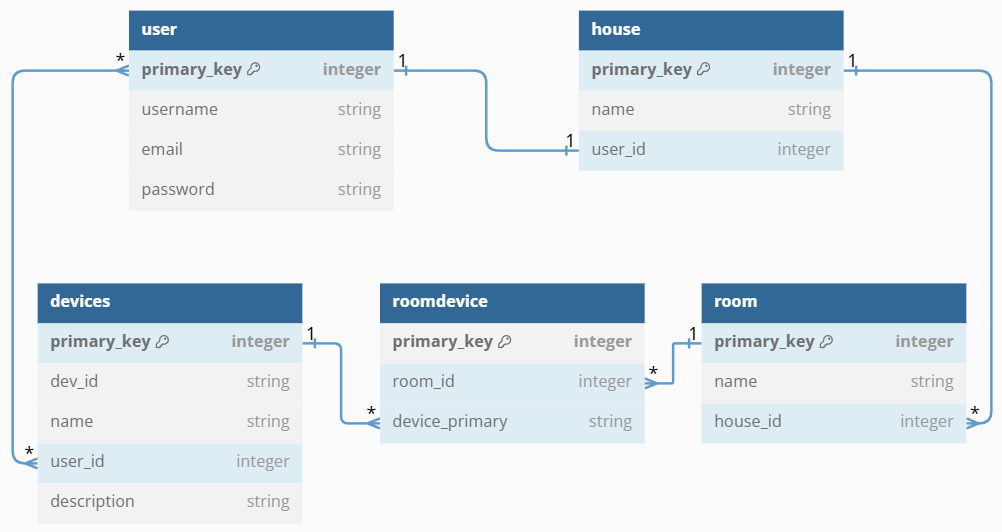
\includegraphics[width=\textwidth]{datenbank.png}
    \caption{Datenbank}
    \label{abb:datenbank}
  \end{figure}
  \begin{itemize}
    \item \textbf{user} --- Enthält die Benutzerdaten.
                        \begin{itemize}
                          \item \textit{\textbf{primary\_key:}} Ein Primärschlüssel vom Typ Integer, der automatisch inkrementiert wird.
                          \item \textit{\textbf{username:}} Der Benutzername, der für jeden Benutzer eindeutig ist.
                          \item \textit{\textbf{email:}} Die E-Mail-Adresse des Benutzers, ebenfalls einzigartig.
                          \item \textit{\textbf{password:}} Das Passwort des Benutzers, das verschlüsselt gespeichert wird.
                        \end{itemize}
                        Ein Benutzer kann mehrere Häuser und Geräte haben.
    \item \textbf{house} --- Speichert die vom Benutzer erstellten Häuser. 
                        \begin{itemize}
                          \item \textit{\textbf{primary\_key:}} Ein Primärschlüssel vom Typ Integer, der automatisch inkrementiert wird.
                          \item \textit{\textbf{name:}} Der vom Benutzer erstellte Name des Hauses.
                          \item \textit{\textbf{user\_id:}} Ein Fremdschlüssel, der auf den Primärschlüssel der Tabelle user verweist, um anzugeben, welchem Benutzer das Haus gehört.
                        \end{itemize}
                        Ein Haus gehört zu einem bestimmten Benutzer. Ein Haus kann mehrere Räume enthalten.
    \item \textbf{room} --- Speichert die vom Benutzer erstellten Räume. 
                        \begin{itemize}
                          \item \textit{\textbf{primary\_key:}} Ein Primärschlüssel vom Typ Integer, der automatisch inkrementiert wird.
                          \item \textit{\textbf{name:}} Der vom Benutzer erstellte Name des Raums.
                          \item \textit{\textbf{house\_id:}} Ein Fremdschlüssel, der auf den Primärschlüssel der Tabelle house verweist.
                        \end{itemize}
                        \par Ein Raum gehört immer zu einem bestimmten Haus. Ein Raum kann mehrere Geräte enthalten.
    \item \textbf{devices} --- Speichert die vom Benutzer angemeldeten Geräte. 
                        \begin{itemize}
                          \item \textit{\textbf{primary\_key:}} Ein Primärschlüssel vom Typ Integer, der automatisch inkrementiert wird.
                          \item \textit{\textbf{dev\_id:}} Die eindeutige, vordefinierte ID des Geräts. 
                          \item \textit{\textbf{name:}} Der vom Benutzer erstellte Name des Geräts.
                          \item \textit{\textbf{user\_id:}} Ein Fremdschlüssel, der auf den Primärschlüssel der Tabelle user verweist und angibt, welchem Benutzer das Gerät gehört.
                          \item \textit{\textbf{description:}} Eine optionale Beschreibung des Geräts.
                        \end{itemize}
                        Ein Gerät gehört genau einem Benutzer und einem Raum. Ein anderes Gerät mit derselben Geräte-ID kann jedoch von einem anderen Benutzer angemeldet und einem anderen Raum zugeordnet werden.
    \item \textbf{roomdevice} --- Speichert die Zuordnung der Geräte zu den Räumen. 
                        \begin{itemize}
                          \item \textit{\textbf{primary\_key:}} Ein Primärschlüssel vom Typ Integer, der automatisch inkrementiert wird.
                          \item \textit{\textbf{room\_id:}} Ein Fremdschlüssel, der auf den Primärschlüssel der Tabelle room verweist.
                          \item \textit{\textbf{device\_primary:}} Ein Fremdschlüssel, der auf den Primärschlüssel der Tabelle device verweist.
                        \end{itemize}
  \end{itemize}
  \paragraph{Aufbau mit SQLAlchemy}
  \par \textbf{}
  \par Jetzt müssen diese Tabellen und deren Verknüpfungen in Form der Modellen in SQLAlchemy definiert werden. Die Models sind in der Datei \texttt{models.py} (Listing \ref{lst:dbmodels}) definiert. 
  \par Zunächst müssen die benötigte Module importiert werden. Das Modul \texttt{bcrypt} wird für die Entschlüssertung und Verifizierung der Passwörter verwendet. Die Module aus der Bibliothek \texttt{sqlalchemy} enthalten die Funktion für die Interaktionen mit der Datenbank. Das Modul \texttt{.base} ist die Datei \texttt{base.py} (Lisitng \ref{lst:dbbase}). Da wird nur ein \texttt{declarative\_base} importiert, und in der Variable \texttt{Base} initialisiert. 
  \begin{lstlisting}[frame=single, style=py, numbers=left, label={lst:dbbase}, caption={db: base.py}]
    from sqlalchemy.orm import declarative_base
    Base = declarative_base()
  \end{lstlisting}  
  \par Die Tabellenmodelle werden in Klassen definiert, die von der \texttt{Base} erben. Dies ist die Standardeinstellung für SQLAlchemy. Die Variable \texttt{\_\_tablename\_\_} legt der Name der Tabelle fest. Die Spalten sind als Objekte der Klasse \texttt{Column} mit gegebenen Parametern definiert. Die Klasse \texttt{UserModel} enthält eine Funktion für die Validierung der Passwörter (Zeile 17). Die Funktion bekommt ein Password-String als Parameter und vergleicht dieser mit dem im Modell gespeicherten Passwort.
  \par In SQLAlchemy, wenn ein \texttt{ChlidModel} Modell einen Fremdschlüssel des \texttt{ParentModel} Modells beinhaltet, muss eine Beziehung mit dem \texttt{ChlidModel} Modell in der \texttt{ParentModel} Klasse definiert werden. Dies wird verwendet, um Datenbankkonflikte beim Löschen oder Aktualisieren von Einträgen im Modell \texttt{ChlidModel} zu vermeiden.
  \par Die Klasse \texttt{HouseModel} enthält neben der Definition der Spalten eine Beziehung zwischen \texttt{HouseModel} und \texttt{RoomModel} im Attribut \texttt{rooms}. Die Beziehung ist so definiert, dass alle zugehörigen Räume gelöscht werden, wenn das Haus gelöscht wird. Außerdem ist in der Klassenvariablen \texttt{\_\_table\_args\_\_} mit dem Befehl \texttt{UniqueConstraint('name', 'user\_id')} (Zeile 27) definiert, dass die Kombination der Spalten \texttt{name} und \texttt{user\_id} eindeutig sein muss. Ein Benutzer kann also nicht 2 Häuser mit dem gleichen Namen anlegen.
  \par Die Klassen \texttt{RoomModel} und \texttt{DeviceModel} haben eine Beziehung zur Klasse \texttt{RoomDeviceModel}, und in der Klasse \texttt{RoomDeviceModel} werden die Beziehungen zu den beiden Klassen definiert. Damit wird sichergestellt, dass beim Löschen eines Raumes oder eines Gerätes auch die entsprechende Verknüpfung gelöscht wird. Dabei ist zu beachten, dass beim Löschen eines Raumes das zum Raum gehörende Gerät nicht gelöscht wird und umgekehrt.
  \paragraph{Interaktionen mit der Datenbank}
  \textbf{}
  \par In der Datei \texttt{queries.py} (Listing \ref{lst:dbqueries}) sind die benötigten Funktionen für die Interaktion mit der Datenbank definiert. Diese Funktionen ermöglichen das Einfügen, Löschen, Abrufen und Aktualisieren der Daten in der Datenbank.
  \par Jede Funktion bekommt ein \texttt{AsyncSession} als erster Parameter. Über diese Session werden die Operationen in der Datenbank duchgeführt. Das erlaubt auch asynchroner Zugriff zur Datenbank.
  \par Als Beispiel werde ich die Struktur der Funktion \texttt{add\_user()} näher erläutern. Diese Funktion fügt einen neuen Benutzer in die Datenbank ein. Die Funktion erhält als Parameter \texttt{AsyncSession} und die Benutzerdaten, d.h. Benutzername, Email und Passwort. Zuerst wird das Passwort verschlüsselt. Anschließend wird ein Objekt \texttt{new\_user} der Klasse \texttt{UserModel} mit den übergebenen Parametern erzeugt. Dieses Objekt wird mit dem Befehl \texttt{db\_session.add(new\_user)} in die Datenbank eingefügt. Nach dem Einfügen muss der Befehl \texttt{db\_session.commit()} aufgerufen werden, um die Änderungen in der Datenbank zu speichern. Anschließend wird das \texttt{new\_user} aktualisiert und der Primärschlüssel zurückgegeben.
  \par Beim Arbeiten mit der Datenbank müssen mögliche Fehler behandelt werden. Deshalb enthält jede Funktion einen \texttt{Try-Catch-Block}. 
  \par Ein \texttt{IntegrityError} wird ausgelöst, wenn eine Datenbankoperation gegen eine Integritätsbedingung der Datenbank verletzt. Er wird bei Verletzung einer Fremdschlüsselbeziehung, der Unique Constraints oder beim Einfügen von Daten des falschen Typs erzeugt. 
  \par Ein \texttt{SQLAlchemyError} umfasst alle Fehler, die von SQLAlchemy ausgelöst werden, wenn die Operation nicht erfolgreich war. Dieser Fehler wird bei Syntaxfehlern in der SQL-Abfrage oder bei Fehlern in der Datenbankverbindung ausgelöst.
  \par Alle anderen möglichen Fehler, die keine \texttt{SQLAlchemy}-Fehler sind, werden im Block \texttt{Exception} gesammelt.
  \par Bei jedem Fehler wird der Fehler geloggt und die Session zurückgesetzt, damit keine unvollständigen Daten in der Datenbank gespeichert werden. Anschließend wird eine \texttt{HTTPException} mit Status und Beschreibung des Fehlers zurückgegeben.
  \paragraph{Initialisierung der Datenbank}
  \par \textbf{}
  \par Beim Import des Moduls \texttt{db} wird die Klasse \texttt{\_\_init\_\_} (Listing \ref{lst:dbinit}) aufgerufen. In dieser Klasse wird zunächst der Logger initialisiert. Anschließend wird eine asynchrone Engine \texttt{async\_engine} für die Verbindung zur Datenbank erzeugt. Mit dem Parameter \texttt{async\_engine} wird das Objekt \texttt{async\_session} der Klasse \texttt{Sessionmaker} erzeugt. Die Funktion \texttt{create\_tables()} initialisiert alle Tabellen in den Klassenmodellen, die von der Klasse \texttt{Base} erben. Die Funktion \texttt{get\_session()} gibt eine asynchrone Session aus der \texttt{async\_session} zurück. Mit dieser Session wird dann auf die Datenbank zugegriffen. 
% 
  \subsubsection{Webbasierte Schnittstelle (API)} 
  \par Um die Benutzerinteraktionen mit dem System zu ermöglichen, muss eine Schnittstelle gebaut werden. Diese Schnittstelle muss den gesicherten Zugriff zu dem System bieten, die notwendigen Informationen bereitstellen, auf die Benutzerinteraktionen reagieren und die Daten verwalten. Nach sorgfältiger Abwägung verschiedener Optionen habe ich mich für die Implementierung einer webbasierten Schnittstelle auf Basis von \texttt{FastAPI} entschieden.
  \par Ein entscheidender Vorteil von \texttt{FastAPI} gegenüber anderen Frameworks wie \texttt{Flask} oder \texttt{Django} in diesem Projekt ist die native Unterstützung asynchroner Programmierung. Dadurch kann \texttt{FastAPI} Anfragen effizient bearbeiten, indem sie mehrere Tasks gleichzeitig ausführt, anstatt blockierend auf das Ende einzelner Prozesse zu warten. Dies ist für mein System besonders vorteilhaft, da mehrere Benutzerinteraktionen, Datenverarbeitung und auch MQTT-Kommunikation parallel ablaufen müssen. Darüber hinaus bietet \texttt{FastAPI} automaisch generierte Dokumentation für die API.
  \par Die zentrale Idee hinter der Entwicklung der API besteht darin, dem Benutzer eine effiziente und sichere Möglichkeit zu bieten, IoT-Geräte in einer strukturierten Umgebung zu verwalten. Dies umfasst das Hinzufügen neuer Geräte, die Gruppierung dieser Geräte in Räumen sowie die Verwaltung mehrerer Räume innerhalb eines Hauses. Darüber hinaus ermöglicht die API die kontinuierliche Überwachung und Steuerung der hinzugefügten Geräte.
  \par Der Webserver ist, wie auch anderen Komponenten, in einem Paket namens \texttt{webserver} srukturiert. Die Struktur des Packets ist wie folgt aufgebaut:
  \begin{Verbatim}[frame=single]
    bachelor/code/spa/webserver
    |
    |--- __init__.py
    |--- routes.py
    |--- services.py
    |--- templates/
    |--- static/
  \end{Verbatim}
  
  
  \par Die Kommunikation zwischen Client und Server erfolgt über HTTP-Methoden:
  \begin{itemize}
    \item \textbf{GET}: Zum Abrufen von Informationen aus dem System.
    \item \textbf{POST:} Zum Übermitteln neuer Daten oder Benutzerinteraktionen.
    \item \textbf{PUT:} Zur Aktualisierung vorhandener Informationen. 
    \item \textbf{DELETE:} Zum Löschen von Daten.
  \end{itemize} 
  \par Im Skript \texttt{routes.py} sind die API-Endpunkte definiert, die verschiedene Funktionen des Systems bereitstellen. Jeder Endpunkt ist dabei einer bestimmten Aufgabe zugeordnet. 
  \par Zur besseren Strukturierung und Modularisierung des Codes wurden die Hilfsfunktionen in das Skript \texttt{services.py} ausgelagert. Diese Funktionen enthalten die Anwendungslogik, verarbeiten die Daten und stellen sie zur Verfügung, verwalten die Verbindungen zum WebSocket.
  \par Nach dem Import der erforderlichen Module wird ein Router mit \texttt{APIRouter()} erstellt, um die API-Endpunkte zu definieren. Der Router wird anschließend mit der Methode \texttt{include\_router()} in das Hauptobjekt der FastAPI-Anwendung integriert.
  \par Um auf Anfragen mit HTML-Dateien zu antworten, wird ein \texttt{Jinja2Templates}-Objekt erstellt. Dabei wird der Pfad zum Ordner \texttt{templates/} angegeben, der die HTML-Vorlagen enthält. Dieses Objekt ermöglicht es, dynamische HTML-Antworten zu generieren, indem Daten aus den Endpunkten in die Vorlagen eingebunden werden.
  \par Jede Funktion, die auf die Datenbank zugreift, benötigt als Parameter eine Instanz der Klasse \texttt{AsyncSession}. Im Modul \texttt{routes.py} wird dazu die Funktion \texttt{get\_session()} aus dem Paket \texttt{db} importiert, die für die Erstellung und Verwaltung von Datenbanksitzungen zuständig ist. Durch die Verwendung des Abhängigkeitsmechanismus \texttt{Depends(get\_session)} wird bei jedem Aufruf einer Router-Funktion automatisch eine neue Datenbanksitzung erzeugt und an die entsprechenden Unterfunktionen weitergegeben. Dies ermöglicht eine effiziente und asynchrone Kommunikation mit der Datenbank, wodurch mehrere Anfragen gleichzeitig ohne blockierende Wartezeiten bearbeitet werden können.
  \par Durch die Verwendung von FastAPI-Routern und einer klar strukturierten Modulanordnung bleibt die API übersichtlich, leicht wartbar und erweiterbar. Die Trennung von Präsentationslogik (HTML, CSS) und Daten (API) wird ebenfalls gewährleistet.
  \paragraph{Sicherheit}
  \par \textbf{}
  \par Sicherheit spielt bei diesem System eine wichtige Rolle. Für die API gibt es zwei kritische Sicherheitspunkte: die Übertragung sensibler Daten und die Authentifizierung der Benutzer.
  \par Um sensible Daten, wie Passwörter, sicher zu speichern, wird der Algorithmus \texttt{bcrypt} verwendet. Anstatt Passwörter im Klartext zu speichern, wird bei der Registrierung eines Benutzers das Passwort gehasht. Der Hash wird in der Datenbank gespeichert, nicht das Passwort selbst. Bei der Anmeldung wird das eingegebene Passwort mit dem gespeicherten Hash verglichen, ohne dass das Originalpasswort jemals entschlüsselt wird. Dadurch sind die Benutzerdaten auch dann geschützt, wenn die Datenbank kompromittiert wird.
  \par Zur Authentifizierung und Identifizierung des Benutzers nach erfolgreicher Anmeldung wird das JWT-Verfahren\footnote {JSON Web Token} verwendet. Die Funktion \texttt{services.create\_jwt\_token()} generiert ein JWT-Token, das an den Benutzer zurückgegeben wird. Dieses Token enthält die Benutzer-ID in verschlüsselter Form, besitzt eine in der Konfiguration definierte Ablaufzeit (\texttt{Config.JWT\_EXPIRE\_TIME}) und wird mit einem geheimen Schlüssel (\texttt{Config.JWT\_SECRET\_KEY}) signiert.
  \par Das Token muss clientseitig gespeichert und bei jeder Anfrage im HTTP-Header mitgesendet werden, um die Authentifizierung des Benutzers sicherzustellen. Der entsprechende Header muss dabei die folgende Struktur aufweisen:
  \begin{Verbatim}[frame=single]
    headers: {
        "auth": "Bearer <JWT TOKEN>"
    }
  \end{Verbatim}
  \par Das Request-Objekt wird an die Funktion \texttt{routes.get\_token()} übergeben, die das JWT-Token aus dem HTTP-Header extrahiert. Dabei wird geprüft, ob der Header das Feld „\texttt{auth}“ enthält und ob dessen Wert mit dem Schlüsselwort "Bearer" beginnt. Ist dies nicht der Fall, wird eine Exception ausgelöst, da das Token in einem ungültigen Format vorliegt. Im normalen Ablauf wird das Token aus dem Header extrahiert und zur weiteren Verarbeitung zurückgegeben.
  \par Die Verifizierung des Tokens stellt eine grundlegende Voraussetzung für alle API-Funktionen dar. Nur gültige und nicht abgelaufene Tokens ermöglichen den Zugriff auf geschützte Ressourcen der API.
  \par Nach der Extraktion wird das Token als Parameter an die Funktion \texttt{services.verify\_token()} übergeben, um seine Gültigkeit zu überprüfen. Zunächst wird das Token entschlüsselt, und die darin enthaltene Benutzer-ID wird extrahiert.  Ist das Token abgelaufen, ungültig, fehlerhaft oder fehlen notwendige Informationen, wird eine entsprechende Fehlermeldung ausgegeben und eine HTTP-Exception mit dem entsprechenden Statuscode ausgelöst. Andernfalls wird die Benutzerkennung für nachfolgende Verarbeitungsschritte zur Verfügung gestellt.
  \paragraph{Anmeldung}
  \par \textbf{}
  \par Damit ein Benutzer die Funktionen der API nutzen kann, muss zunächst ein Konto erstellt werden. Dies erfolgt durch Senden eines \texttt{POST}-Requests an die Route \texttt{/sign\_up}. Der Request muss die erforderlichen Parameter \texttt{username}, \texttt{email} und \texttt{password} enthalten. Nach Erhalt der Anfrage wird die Funktion \texttt{signup\_post()} aufgerufen, die die eingegebenen Daten verarbeitet und die Benutzerregistrierung durchführt.
  \par Die Registrierungsdaten werden als \texttt{SignUpModel}-Objekt entgegengenommen und an die Funktion \texttt{services.signup\_user()} weitergeleitet. Diese Funktion übernimmt die Validierung der Eingaben, indem sie prüft, ob alle erforderlichen Felder ausgefüllt wurden. Wenn ein Wert fehlt, wird die entsprechende Fehlermeldung geloggt und zurückgegeben. Sind alle Daten vollständig, wird der Benutzer mit der Funktion \texttt{queries.add\_user()} in der Datenbank gespeichert. 
  \par Nach erfolgreicher Speicherung wird ein JWT-Token generiert und zurückgegeben, das die Benutzer-ID enthält. Mit diesem Token kann der Benutzer direkt angemeldet werden. Tritt während des Prozesses eine Exception auf, so wird diese geloggt und eine entsprechende Fehlermeldung ausgegeben.
  \paragraph{Einloggen}
  \par Um einem bereits registrierten Benutzer den Zugriff auf die API zu ermöglichen, ist eine Authentifizierung erforderlich. Diese erfolgt durch das Senden eines \texttt{POST}-Requests an die Route \texttt{/login}. Der Request muss die Parameter \texttt{username} und \texttt{password} enthalten, die im \texttt{user\_data}-Objekt übergeben werden. Nach Erhalt der Anfrage wird die Funktion \texttt{login\_post()} aufgerufen, die die Authentifizierung des Benutzers vornimmt.
  \par Die Benutzerdaten werden als \texttt{UserLoginModel} entgegengenommen und an die Funktion \texttt{services.auth\_user()} übergeben. Diese Funktion überprüft, ob die erforderlichen Felder \texttt{username} und \texttt{password} ausgefüllt wurden. Ist es nicht der Fall, wird eine entsprechende Fehlermeldung ausgegeben. Anschließend wird mit der Funktion \texttt{queries.get\_user\_data()} geprüft, ob ein Benutzer mit dem angegebenen \texttt{username} in der Datenbank existiert. Wird kein entsprechender Datensatz gefunden, wird eine \texttt{HTTPException} mit dem Statuscode \texttt{401} und der Meldung „Invalid username“ ausgelöst.
  \par Wenn der Benutzer existiert, wird das eingegebene Passwort mit der gespeicherten verschlüsselten Version verglichen. Ist die Prüfung erfolgreich, gibt die Funktion den Primärschlüssel zurück. Andernfalls wird die Fehlermeldung „Wrong password“ zurückgegeben.
  \par Nach erfolgreicher Authentifizierung wird in der Funktion \texttt{loin\_post()} ein JWT-Token erzeugt und zurückgegeben, das die Benutzerkennung enthält. Tritt während des Prozesses eine Exception auf, wird diese protokolliert und eine entsprechende Fehlermeldung ausgegeben.
  \par Nach dem erfolgreichen Eingloggen und Erhalt des Tokens, kann der Benutzer zu den Funktionen der API zugreifen. 
  \paragraph{Haus und Raum}
  \par \textbf{}
  \par Der Benutzer kann seine Geräte nach Räumen und die Räume nach Häusern gruppieren. Dies erleichtert die Verwaltung und Überwachung der Geräte. Besonders im Frontend ist dies sehr nützlich, da es eine klare Strukturierung des Hauses geschaffen wird. Dabei kann ein Benutzer mehrere Häuser besitzen.
  \par Um ein Haus zu anzulegen, muss ein \texttt{POST}-Request an die Route \texttt{add\_house} gesendet werden. Der Request muss im Header ein Bearer-Token und im Body den Namen des Hauses enthalten. Nach Erhalt des Requests wird die Funktion \texttt{add\_house\_post()} aufgerufen. Standardmäßig wird das Token validiert, und die Benutzer-ID wird aus dem Token extrahiert, um das Haus dem entsprechenden Benutzer zuzuordnen. Wenn eine gültige Benutzer-ID aus dem Token erzeugt wurde, wird diese zusammen mit der Instanz der Klasse \texttt{AsyncSession} und dem Namen des Hauses an die Funktion \texttt{services.create\_new\_house()} übergeben.
  \par Die Funktion \texttt{services.create\_new\_house()} prüft zunächst, ob ein gültiger Hausname übergeben wurde. Anschließend wird mit der Funktion \texttt{queries.add\_new\_house()} ein neuer Eintrag in der Datenbank angelegt und dem Benutzer zugeordnet. Wenn die Erstellung erfolgreich war, gibt die Funktion eine Bestätigung zurück. Andernfalls oder im Fehlerfall wird eine entsprechende Fehlermeldung generiert und geloggt.
  \par Das Verfahren zum Hinzufügen eines Raumes zu einem House ist im Wesentlichen dasselbe wie bei der Erstellung eines House. An die Route \texttt{add\_room} wird ein \texttt{POST}-Request mit dem Token im Header und mit dem Namen des Raumes sowie der zugehörigen House-ID als \texttt{RoomModel} im Inhalt gesendet. Auch hier wird das JWT-Token standardmäßig validiert, und die Benutzer-ID daraus extrahiert. 
  \par Die Daten des Raumes und die Benutzer-ID werden an die Funktion \texttt{services.add\_room()} übergeben. Diese Funktion holt zunächst mit dem Befehl \texttt{queries.get\_house()} die Daten des Hauses aus der Datenbank, um den Besitzer des Hauses zu bestätigen. Stimmt die übergebene Benutzer-ID mit der in der Datenbank gespeicherten Benutzer-ID des Hausbesitzers überein, wird mit der Funktion \texttt{queries.add\_new\_room()} ein neuer Eintrag in der Datenbank erstellt. Im Erfolgsfall wird eine Bestätigung zurückgegeben. 
  \par Wenn der Benutzer nicht berechtigt ist, einen Raum zu dem angegebenen Haus hinzuzufügen, wird eine Meldung über unberechtigten Zugriff geloggt und als Fehlerantwort zurückgegeben.
  Das Löschen eines Hauses oder Raumes erfolgt ähnlich wie das Hinzufügen: Es wird ein \texttt{POST}-Request an die entsprechenden Routen (\texttt{/delete\_house} bzw. \texttt{delete\_room}) gesendet, wobei im Header das Bearer-Token und im Inhalt des Requests die zu löschende Haus- bzw. Raum-ID übermittelt wird. Dabei ist zu beachten, dass beim Löschen eines Hauses auch alle zugehörigen Räume gelöscht werden. Dies wird durch die Beziehung \texttt{rooms} in \texttt{HouseModel} in der Datenbank definiert. 
  \par Beim Löschen eines Hauses wird ein Request mit den Benutzer- und House-ID an die Route \texttt{/delete\_house} gesenden. Nach der Validierung des Tokens und Erzeugeung der Benutzer-ID werden die Daten an die Funktion \texttt{services.delete\_house()} übergeben. Diese Funktion prüft, ob das Haus dem Benutzer gehört und löscht mit dem Befehl \texttt{queries.delete\_house()} den zugehörigen Eintrag aus der Datenbank. Die zugehörigen Räume werden ebenfalls gelöscht. Im Fehlerfall wird der entsprechende Fehler geloggt und ausgegeben. 
  \par Das Löschen eines Raumes ist ähnlich dem Löschen eines Hauses. Ein Request mit der Raum- und Haus-ID wird an die Route \texttt{delete\_room} gesendet. Nach der Validierung des Tokens und Erzeugeung der Benutzer-ID werden die Daten an die Funktion \texttt{services.delete\_room()} übergeben. Wenn der Benutzer der Eigentümer des Hauses mit der übergebenen House-ID ist, wird der Raum aus der Datenbank gelöscht. Tritt ein Fehler auf, wird dieser geloggt und die entsprechende Meldung wird ausgegeben.
  \par Die Route \texttt{/get\_houses} gibt alle Häuser des Benutzers im JSON-Format zurück. Der Request muss im Header nur das Token enthalten, aus dem die Benutzer-ID erzeugt wird. Die Benutzer-ID wird an die Funktion \texttt{services.get\_houses()} übergeben, die Benutzer-ID an die Funktion \texttt{queries.get\_houses\_on\_user()} übergibt. Diese Funktion gibt eine Liste von \texttt{HouseModel} zurück, die dem Benutzer gehören. Diese Liste wird in eine „List of Dictionaries“ umgewandelt, die alle Häuser, die zugehörigen Räume und die Geräte enthält. Anschließend wird ein JSONResponse-Objekt zurückgegeben.
  \paragraph{Device}
  \par \textbf{}
  \par Die zentrale Aufgabe der API ist die Überwachung der angeschlossenen Geräte und die Benachrichtigung der Benutzer über erkannte Gefahren. Damit dieses System genutzt werden kann, muss der Benutzer die Möglichkeit haben, seine Geräte in das System einzubinden.
  \par Jedes Gerät verfügt über eine eindeutige Geräte-ID, die im Programmcode des Gerätes fest hinterlegt ist und zur Identifikation innerhalb des Systems dient. Die Speicherung der Geräte erfolgt in der Datenbank innerhalb der Tabelle \texttt{device} in Form von \texttt{DeviceModel}-Objekten.
  \par Die Integration eines neuen Gerätes erfolgt durch das Senden eines \texttt{POST}-Requests an die Route \texttt{/add\_new\_device}. Der Header des Requests muss ein gültiges JWT-Token enthalten, aus dem die Benutzer-ID ausgelesen wird. Im Body des Requests muss die eindeutige Geräte-ID angegeben werden.  Optional kann ein vom Benutzer erstellter Name und eine Beschreibung des Gerätes sowie die Raum-ID für die Zuordnung des Gerätes zum Raum übergeben werden. Der Name dient ausschließlich der Benutzerfreundlichkeit, indem er eine eindeutige Identifikation des Gerätes ermöglicht. Die übergebenen Daten werden innerhalb der API als Instanz \texttt{services.DeviceModel} entgegengenommen und verarbeitet.
  \par Nach Erhalt des Requests wird die Funktion \texttt{add\_new\_device\_post} aufgerufen. Zuerst wird das Token validiert und die Benutzer-ID aus dem Token erzeugt. Anschließend werden die Gerätedaten an die Funktion \texttt{services.add\_new\_device} übergeben. Diese prüft zunächst, ob sowohl die Geräte-ID als auch der Gerätename im Request enthalten sind. Fehlt eine dieser Angaben, wird der Vorgang abgebrochen und eine Fehlermeldung zurückgegeben.
  \par Zusätzlich hat der Benutzer die Möglichkeit, das Gerät direkt einem bestimmten Raum innerhalb des Hauses zuzuordnen. Dazu muss im Body des Requests die entsprechende Raum-ID angegeben werden. Die Funktion \texttt{services.add\_new\_device} sucht in diesem Fall, mit dem Befehl \texttt{queries.get\_house\_by\_room} nach dem entsprechenden Haus. Anschließend wird geprüft, ob die aus dem Token extrahierte Benutzer-ID mit der des Hauseigentümers übereinstimmt. Ist dies nicht der Fall, wird der Zugriff verweigert, der Vorgang abgebrochen und eine entsprechende Fehlermeldung zurückgegeben.
  \par Anschließend wird mit dem Befehl \texttt{queries.add\_new\_device} das Gerät zunächst ohne direkte Raumzuordnung in der Datenbank gespeichert. Ist eine Raum-ID vorhanden, wird mit dem Befehl \texttt{queries.add\_room\_device} ein Eintrag in der Tabelle \texttt{roomdevice} erzeugt, der den Primärschlüssel des Gerätes mit der Raum-ID verknüpft.
  \par Diese strukturierte Vorgehensweise gewährleistet nicht nur eine sichere und konsistente Registrierung neuer Geräte, sondern bietet dem Benutzer auch die Möglichkeit, seine Smart-Home-Geräte flexibel zu verwalten und eindeutig zu identifizieren.
 \paragraph{MQTT-Client}
 \par Die Geräte senden ihre Daten über die MQTT-Verbindung an dem MQTT-Broker. Dabei hat jedes Gerät ein separates Topic, das sich auf die Geräte-ID bezieht. Um die Daten von dem Gerät zu erhalten muss ein MQTT-Client das Topic abonnieren.
 \par Der MQTT-Client für den Webserver ist im Paket \texttt{mqtt} eingepackt. 
 \par Der MQTT-Client 
  \subsubsection{Frontend}
  \subsubsection{Integration der Komponenten}
  \par MQtt client, erhalten Daten von Broker etc

\newpage
\section{Funktionsweise des Systems}
\par Hier wird beschrieben wie der Benutzer das System verwendet und wie laufen die Prozesse im System. Es wird ein Diagramm ersetellt ähnlich zu im PA 2. 
\section{Ergebnisse und Diskussion}
\par Hier wird zusammengefasst, was ich mit diesem Projekt gelernt habe, welche Ziele erreicht und nicht erreicht habe, mögliche Weiterentwicklung des Systems etc
\newpage
\section{Quellen}
\begin{thebibliography}{20}
  \bibitem{pa1}
  O. Baida,
  \textit{Anbindung der Sensoren und Aktoren an den Arduino zur Realisierung eines Sicherheitssystems},
  Projektarbeit 1, 2024.

  \bibitem{pa2}
  O. Baida, Projektarbeit 2 \textit{Sicherheitssystem fur das Haus basierend auf Arduino, ESP8266 \& Raspberry Pi} \url{https://github.com/oleksiibaida/PA2.git}
  \bibitem{video}
  
  \bibitem{statita_smhomes}
  Statista, \textit{„Smart Home - Anzahl der Haushalte in Deutschland 2028“}, Zugegriffen: 13. Januar 2025. [Online]. Verfügbar unter \url{https://de.statista.com/prognosen/885611/anzahl-der-smart-home-haushalte-in-deutschland}
  \bibitem{spiegel_heizung}
  J. Breithut, \textit{„Strom und Heizung: Wann ein Smart Home wirklich beim Energiesparen hilft“}, Der Spiegel, 17. Juli 2022. Zugegriffen: 13. Januar 2025. [Online]. Verfügbar unter: \url{https://www.spiegel.de/netzwelt/gadgets/strom-und-heizung-wann-ein-smart-home-wirklich-beim-energiesparen-hilft-a-ffb4b710-0cec-40e4-a2c4-6c5d4a3feb92}


  \par \textbf{Links zur verwendeten Hardware:}
  \bibitem{arduino}
  Arduino.cc, \textit{Arduino UNO}, \url{https://docs.arduino.cc/hardware/uno-rev3/}
  \bibitem{raspi}
  Raspberry Pi Foundation, \textit{Raspberry Pi 1 B+}, \url{https://www.raspberrypi.com/products/raspberry-pi-1-model-b-plus/}
  \bibitem{esp8266}
  Espressif, \textit{ESP8266}, \url{https://www.espressif.com/}, \url{https://www.electronicwings.com/sensors-modules/esp8266-wifi-module}

  \bibitem{bme680}
  Bosh, \textit{BME680 - Datasheet}, \url{https://www.bosch-sensortec.com/media/boschsensortec/downloads/datasheets/bst-bme680-ds001.pdf}, Zugriff: 4. Februar 2025.

  \bibitem{vcnl4040}
  Vishay, \textit{VCNL4040 - Datasheet}, \url{https://www.vishay.com/docs/84274/vcnl4040.pdf}, Zugriff: 5. Februar 2025.

  \par \textbf{Links zur verwendeten Software:}
  \bibitem{mqtt}
  Dr Andy Stanford-Clark, Arlen Nipper, \textit{Message Queuing Telemetry Transport}, \url{https://mqtt.org/}
  \bibitem{python}
  Guido van Rossum, Python Software Foundation, \textit{Python}, \url{https://www.python.org/}
  \bibitem{telegram}
  Telegram FZ-LLC, \textit{Telegram Messenger}, \url{https://github.com//telegramdesktop/tdesktop}
  \par \textbf{Linux-Packete}:
  \bibitem{hostapd}
  Jouni Malinen, \textit{hostapd}, \url{https://w1.fi/hostapd/}, Zugriff am: 19. September 2024.
  \bibitem{dnsmasq}
  Simon Kelley, \textit{dnsmasq}, \url{https://dnsmasq.org/doc.html}, Zugriff am: 20. September 2024.
  \bibitem{mosquitto}
  Eclipse Foundation, \textit{Eclipse Mosquitto}, \url{https://mosquitto.org/}
  \par \textbf{ESP- und Arduino-Bibliotheken}
  \bibitem{pubsub} 
  Knolleary, \textit{PubSubClient}, \url{https://pubsubclient.knolleary.net/}, Zugriff am: 21. Oktober 2024.
  \bibitem{espwifi}
  ESPWIFI.h, \url{https://arduino-esp8266.readthedocs.io/en/latest/esp8266wifi/readme.html}
  \bibitem{eeprom}
  EEPROM.h, \url{https://docs.arduino.cc/learn/built-in-libraries/eeprom/}
  \bibitem{keypad}
  Keypad.h \url{https://docs.arduino.cc/libraries/keypad/}
  \bibitem{scholz}
  R. Scholz, \textit{Syncloop}, Persönliche Mitteilungen
  \par \textbf{Python-Bibliotheken}
  \bibitem{paho}
  Pierre Fersing, Roger Light \textit{paho-mqtt}, \url{https://pypi.org/project/paho-mqtt/}, Zugriff am: 21. Oktober 2024.
  \bibitem{tgbot}
  Open Source, \textit{python-telegram-bot}, \url{https://docs.python-telegram-bot.org/en/v21.6/}
  \bibitem{json}
  Python Software Foundation, \textit{json}, \url{https://docs.python.org/3/library/json.html}
  \bibitem{threading}
  Python Software Foundation, \textit{threading}, \url{https://docs.python.org/3/library/threading.html}
  \bibitem{queue}
  Python Software Foundation, \textit{queue}, \url{https://docs.python.org/3/library/queue.html}
  \bibitem{sqlite}
  Gerhard Häring, \textit{sqlite3}, \url{https://docs.python.org/3/library/sqlite3.html}
  \bibitem{pyzbar}
  Lawrence Hudson, \textit{pyzbar}, \url{https://github.com/NaturalHistoryMuseum/pyzbar/}
  \bibitem{cv2}
  Intel, \textit{OpenCV}, \url{https://github.com/opencv/opencv-python}
  \bibitem{aiohttp}
  Aio-Libs, \textit{aiohttp}, \url{https://github.com/aio-libs/aiohttp}
\end{thebibliography}



\listoffigures
\addcontentsline{toc}{section}{Abbildungsverzeichnis}

\listoftables
%\addcontentsline{toc}{section}{Tabellenverzeichnis}
% \lstlistoflistings
% \addcontentsline{toc}{section}{Programmcode}
\newpage
\section{Programmcode}

% \begin{lstlisting}[frame=single, style=cpp, numbers=left, label={lst:esp8266setup}, caption={ESP: setup}]
%   void setup()
%   {
%     Serial.begin(9600);
%     // GET WiFi Daten aus EEPROM
%     EEPROM.begin(128);
%     char eeprom_ssid[MAX_SSID_LENGTH] = {0};
%     char eeprom_password[MAX_PASSWORD_LENGTH] = {0};
%     EEPROM.get(0, eeprom_ssid);
%     EEPROM.get(32, eeprom_password);
%     EEPROM.end();
%     // Daten gefunden
%     if (is_valid_string(eeprom_ssid, MAX_SSID_LENGTH) && is_valid_string(eeprom_password, MAX_PASSWORD_LENGTH))
%     {
%       if (connect_wifi(eeprom_ssid, eeprom_password))
%       {
%         connect_mqtt();
%         return;
%       }
%     }
%     // keine WLAN-DAten gefunden
%     setup_ap();
%   }
% \end{lstlisting}
% \begin{lstlisting}[frame=single, style=cpp, numbers=left, label={lst:esp8266validstring}, caption={ESP: is\_valid\_string}]
%   bool is_valid_string(char *data, int max_length)
%   {
%     if (strlen(data) == 0 or strlen(data) > max_length)
%       return false;
%     for (int i = 0; i < max_length; i++)
%     {
%       if (data[i] == '\0')
%         return true; // End of valid String
%       if (data[i] == 0xFF) // Default EEPROM
%         return false;
%     }
%     return false;
%   }
% \end{lstlisting}
% \begin{lstlisting}[frame=single, style=cpp, numbers=left, label={lst:espconnectwifi}, caption={ESP: connect\_wifi}]
%   bool connect_wifi(char *ssid, char *password)
%   {
%     WiFi.mode(WIFI_STA);
%     WiFi.begin(ssid, password);
  
%     for (uint8_t i = 0; i < wifi_repeat; i++)
%     {
%       if (WiFi.status() == WL_CONNECTED)
%       {
%         Serial.println(WiFi.localIP());
%         return true;
%       }
%       delay(1000);
%     }
%     return false;
%   }
% \end{lstlisting}
% \begin{lstlisting}[frame=single, style=cpp, numbers=left, label={lst:espconnectmqtt}, caption={ESP: connect\_mqtt}]
%   void mqtt_connect()
%   {
%     set_topics();
%     mqttClient.setServer(MQTT_BROKER_ADRRESS, MQTT_PORT);
%     mqttClient.setCallback(callback);
%     for (int i = 0; i < wifi_repeat; i++)
%     {
%       if (mqttClient.connect(DEVICE_ID))
%         mqttClient.subscribe(SUBSCRIBE_TOPIC);
%         return;
%       else
%         delay(1000);
%     }
%   }
% \end{lstlisting}
% \begin{lstlisting}[frame=single, style=cpp, numbers=left, label={lst:espsettopics}, caption={ESP: set\_topics}]
%   void set_topics()
%   {
%     SUBSCRIBE_TOPIC = (char *)malloc(strlen(TOPIC_COMMAND) + strlen(DEVICE_ID) + 2);
%     PUBLISH_TOPIC = (char *)malloc(strlen("data") + strlen(DEVICE_ID) + 2);
  
%     strcpy(SUBSCRIBE_TOPIC, TOPIC_COMMAND);
%     strcat(SUBSCRIBE_TOPIC, "/");
%     strcat(SUBSCRIBE_TOPIC, DEVICE_ID);
  
%     strcpy(PUBLISH_TOPIC, "data");
%     strcat(PUBLISH_TOPIC, "/");
%     strcat(PUBLISH_TOPIC, DEVICE_ID);
%   }
% \end{lstlisting}
% \begin{lstlisting}[frame=single, style=cpp, numbers=left, label={lst:esp8266defap}, caption={ESP8266: ap\_konfiguration}]
%   const char AP_SSID[] = "ESP8266";
%   const char AP_PASSWORD[] = "setupesp";
%   IPAddress ap_ip(10, 0, 0, 1);
%   IPAddress ap_gateway(10, 0, 0, 1);
%   IPAddress ap_subnet(255, 255, 255, 0);
%   AsyncWebServer server(80);
%   const String html_page = R"rawliteral(
%     <html>
%     <body>
%       <h2>Wi-Fi Configuration</h2>
%       <form action="/save" method="POST">
%         SSID:<br>
%         <input type="text" name="ssid" required><br>
%         Password:<br>
%         <input type="password" name="password" required><br><br>
%         <input type="submit" value="Submit">
%       </form>
%     </body>
%     </html>
%   )rawliteral";
% \end{lstlisting}
% \begin{lstlisting}[frame=single, style=cpp, numbers=left, label={lst:esp8266setupap}, caption={ESP: setup\_ap}]
%   void setup_ap()
%   {
%     WiFi.mode(WIFI_AP);
%     WiFi.softAP(AP_SSID, AP_PASSWORD);
%     WiFi.softAPConfig(ap_ip, ap_gateway, ap_subnet);
  
%     server.on("/", HTTP_GET, [](AsyncWebServerRequest *request)
%               { request->send(200, "text/html", html_page); });
  
%     server.on("/save", HTTP_POST, [](AsyncWebServerRequest *request)
%               {
%                 // get input data
%                 String ssid = request->getParam("ssid", true)->value();
%                 String password = request->getParam("password", true)->value();
%                 if (ssid.length() > MAX_SSID_LENGTH - 1 || password.length() > MAX_PASSWORD_LENGTH - 1)
%                 {
%                   return;
%                 }
%                 // String in char[]
%                 char new_ssid[MAX_SSID_LENGTH] = {0};
%                 strncpy(new_ssid, ssid.c_str(), MAX_SSID_LENGTH - 1);
%                 char new_password[MAX_PASSWORD_LENGTH] = {0};
%                 strncpy(new_password, password.c_str(), MAX_PASSWORD_LENGTH - 1);
  
%                 // in EEPROM speichern
%                 EEPROM.begin(128);
%                 EEPROM.put(0, new_ssid);
%                 EEPROM.put(32, new_password);
%                 EEPROM.commit();
%                 EEPROM.end();
  
%                 request->send(200, "text/html", "WiFi saved. Rebooting...");
%                 ESP.restart(); });
  
%     server.begin();
%   }
% \end{lstlisting}

% \begin{lstlisting}[frame=single, style=cpp, numbers=left, label={lst:esp8266readserial}, caption={ESP8266: readSerialData}]
%   void readSerialData()
%   {
%     if (Serial.available() > 0)
%     {
%       String readString = "";
%       // Lese Daten aus Serial als String ab
%       readString = Serial.readStringUntil('\n');
%       if (sizeof(readString) > buss_serial)
%         return;
%       // String in char-Feld konvertieren
%       char readSerialChar[readString.length() + 1];
%       readString.toCharArray(readSerialChar, readString.length() + 1);    
%       // Suche Position von ':'
%       char *delim_pos = strchr(readSerialChar, ':');
%       if (delim_pos != NULL)
%       {
%         size_t topic_length = delim_pos - readSerialChar;
%         char topic[topic_length + 1];
%         strncpy(topic, readSerialChar, topic_length);
%         topic[topic_length] = '\0';
%         char *message = delim_pos + 1;
%         PUBLISH_TOPIC = (char *)malloc(strlen(CLIENT_ID) + strlen(topic) + 2);
%         if (PUBLISH_TOPIC == NULL)
%         {
%           PUBLISH_TOPIC = topic;
%         }
%         else
%         {
%           strcpy(PUBLISH_TOPIC, topic);
%           strcat(PUBLISH_TOPIC, "/");
%           strcat(PUBLISH_TOPIC, CLIENT_ID);
%         }
%         // MQTT-Nachricht senden
%         mqttClient.publish(PUBLISH_TOPIC, message);
%       }
%       else // kein : gefunden
%         return;
%     }
%   }
% \end{lstlisting}

% \begin{lstlisting}[frame=single, style=cpp, numbers=left, label={lst:esp8266callback}, caption={ESP8266: callback}]
%   void callback(char *topic, byte *payload, unsigned int length)
%   {
%     String id = String(topic).substring(String(topic).indexOf('/') + 1);
%     if (id == CLIENT_ID)
%     {
%       String text = "";
%       for (int i = 0; i < length; i++)
%       {
%         text += (char)payload[i];
%       }
%       text.trim();
%       // Print in Arduino
%       Serial.println(text);
%     }
%   }
% \end{lstlisting}

%


\end{document}
% „“ 